\documentclass[letterpaper]{article}
\usepackage[submission]{aaai2027}
\usepackage[hyphens]{url}
\usepackage{graphicx}
\urlstyle{rm}
\def\UrlFont{\rm}
\usepackage{natbib}
\usepackage{caption}
\usepackage{cuted}
\frenchspacing
\usepackage{amsmath}
\usepackage{amssymb}
\usepackage{booktabs}
\usepackage{multirow}
\usepackage{tikz}
\usepackage{dblfloatfix}
\usetikzlibrary{arrows.meta,positioning,calc,fit}
\pdfinfo{
/TemplateVersion (2027.1)
}
\setcounter{secnumdepth}{0}

\title{Latent Bridge Matching for IDT-Calibrated Style-ID Transfer}
\author{Anonymous Submission}
\affiliations{}
\begin{document}
\maketitle

\begin{abstract}
Art-to-art transfer is easy to fake: when the source is already artwork, the unchanged image can score highly for many requested target styles. Raw style-affinity therefore overstates target-style control. We make this failure explicit with identical-image transfer (IDT) calibration on Distinct5-WikiArt and evaluate style movement only above the unchanged-image floor. We then introduce \emph{Latent Bridge Matching} (LBM), a compact style-ID latent transport family trained by endpoint pairing, a style-conditioned latent field, and terminal distribution matching in VAE space. Inference receives only the source image and target style identifier. On Distinct5-WikiArt, IDT calibration reveals a broad failure zone that engulfs reproduced compact baselines, while LBM forms a usable frontier above it. LBM-K clears the calibrated floor after 1.2 minutes on an RTX 3060, the promoted LBM-Knee point reaches 0.7102 transfer CLIP-S at 0.5397 content preservation, and Pattern+Stokes successors push style into the 0.72--0.73 band. Artifact-sensitive diagnostics and a held-out non-CLIP probe separate the closed Knee point from the style-ceiling row. IDT calibration is therefore necessary, and compact latent transport is sufficient to produce a practical style-ID frontier on consumer GPUs.
\end{abstract}

\begin{strip}
\centering
\vspace{-4mm}
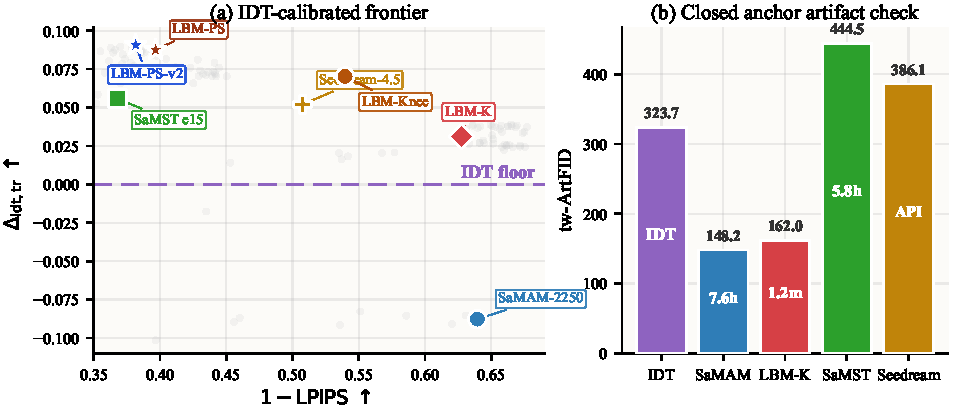
\includegraphics[width=0.965\textwidth]{figures/fig_distinct5_page1_summary.pdf}
\captionof{figure}{Distinct5-WikiArt is not a single-score benchmark. Panel (a) shows the actual decision surface: a large IDT failure zone below zero style gain, and a usable LBM frontier above it. Gray dots are retained development checkpoints; colored markers are the headline rows, including the latent negatives. Panel (b) keeps the same shortlist under aligned all-pairs target-pooled tw-ArtFID, exposing the artifact cost of that frontier. Train time is printed inside each bar.}
\label{fig:distinct5_page1}
\vspace{-5mm}
\end{strip}

\section{Introduction}
Domain-level artistic transfer asks for a target \emph{style identity}, not a target exemplar. That setting creates an immediate evaluation failure: when the source image is already artwork, the unchanged image can already score highly for the requested target style. A method can therefore look strong simply by staying inside a broad art manifold. We make this failure explicit with identical-image transfer (IDT) calibration and report only style gain above the unchanged-image floor. Figure~\ref{fig:distinct5_page1} shows the result immediately: a large failure zone below IDT and a compact frontier above it.

This regime is stricter than reference-guided stylization and lighter than large-prior editing. Inference receives only a source image and a target style identifier, with no exemplar, per-image optimization, or large-prior adaptation. The question is whether a compact style-ID model can still produce reliable target-style motion under that contract.

We answer yes with \emph{Latent Bridge Matching} (LBM), a compact VAE-space transport family built from training-side endpoint pairing, a style-conditioned latent field, and terminal distribution matching with kinetic control. On Distinct5-WikiArt, LBM forms a real frontier: minute-scale anchors clear the IDT floor, LBM-Knee closes the strongest style-cleanliness tradeoff, and Pattern+Stokes successors extend the style ceiling. The paper makes three concrete claims: IDT calibration is necessary; compact style-ID transport works without exemplars or large-prior adaptation; and Distinct5-WikiArt exposes a measurable frontier rather than a single winner.

\section{Related Work}
Most style-transfer systems solve a different inference contract: they either consume a target exemplar or inherit a strong pretrained generator at test time \cite{gatys2016image,huang2017adain,deng2022stytr2,hong2023aespa,huang2024aesfa,zhang2024artbank,chung2024styleid}. Our setting keeps only the target style identity, placing it closest to compact multi-style baselines such as SaMST, Mamba-ST, and SaMam \cite{liu2024samst,botti2025mambast,liu2025samam}. The nearest transport-side analogy is low-energy one-step editing \cite{lu2026chordedit}, although that line targets prompt-conditioned semantic editing rather than domain-level style-ID transfer.

Evaluation is also different. Automatic stylization metrics are unstable and only partially aligned with human judgment \cite{zhou2024comprehensiveeval,yeh2020calibrated,wright2022artfid}, and in art-to-art transfer they reward the unchanged image far too easily. We therefore make the no-op floor explicit and report $\Delta_{\mathrm{idt}}$ before broader plausibility or artifact diagnostics. Full related-work detail is deferred to the supplement.

\section{Method}
\subsection{Inference contract}
LBM is an endpoint transport model in VAE latent space for domain-level artistic transfer. Figure~\ref{fig:distinct5_page1} established the target: clear the IDT floor without paying the artifact cost of the strongest high-style baselines. Figure~\ref{fig:framework} shows the contract used to trace that frontier: style-ID control on top, the active latent transport path in the middle, and endpoint construction plus terminal matching only on the training side. For Distinct5-WikiArt, the source latent is $z_0 \in \mathbb{R}^{4 \times 64 \times 64}$; the historical CycleGAN-256 packet uses $4 \times 32 \times 32$ latents. At inference, the model receives only the source image and target style identifier. Target-domain latents remain training-side supervision only.

Our OT view is deliberately limited and practical. As in recent low-energy transport views of one-step editing \cite{lu2026chordedit}, OT is used as supervisory geometry, not as an online solver claim. In the reproduced Distinct5 mainline, the active headline rows use endpoint-mode OMF rather than the earlier random-time flow residual:
\begin{equation}
    \hat v = v_\theta(z_0,1,s), \qquad \hat z_1 = z_0 + \hat v,
\end{equation}
with active objective
\begin{equation}
    \mathcal{L}_{\mathrm{active}} =
    \lambda_{\mathrm{term}}\mathcal{L}_{\mathrm{term}}(\hat z_1)
    + \lambda_{\mathrm{kin}}\|\hat v\|_2^2,
    \label{eq:active_distinct5_loss}
\end{equation}
where the pairing cache selects terminal targets and the parent flow residual is disabled in the headline rows ($w_{\mathrm{flow}}=0$). We therefore describe the headline Distinct5 family as pairing-cache / terminal-SWD / kinetic OMF.

\subsection{Training-side endpoint construction and latent execution}
We train directly on precomputed VAE latents without paired supervision. For each source latent $z_0$ and target style $s$, the pairing cache exposes a selector-restricted candidate set $\mathcal{C}(z_0,s)$ from the target domain. The terminal target $\tilde z_1$ is drawn from that scheduled set, and the successor family stabilizes it with barycentric targets and queue-side target smoothing. Endpoint pairing therefore decides \emph{where} the model should move; the latent field still learns \emph{how} to execute that move.

Execution is handled by a time-conditioned latent backbone with sinusoidal time embeddings, style spatial priors, and semantic cross-attention. The tokenizer receives only the target style identifier and produces a compact control code $c_s$; the style-conditioned latent field then decides how much motion is needed under the current content.

The endpoint is then regularized by semantic-aligned sliced Wasserstein distance. Let $\Phi_\theta(z_0,s)$ denote the Euler-integrated endpoint. The terminal objective is
\begin{equation}
    \mathcal{L}_{\mathrm{term}} =
    \mathrm{SWD}_1\bigl(\Phi_\theta(z_0,s),\,\tilde z_1\bigr),
\end{equation}
where sorted one-dimensional projections compare generated endpoint patches against target-style patches without requiring spatial correspondence. In the current SA-SWD instantiation, projection directions are chosen from the same routing signal that injects style into the backbone, keeping target-style pressure distributional rather than pointwise. The supplement gives bounded design-grounding support for the active field/solver regime: a local path-action justification for endpoint kinetic regularization and the expected $O(1/K)$ Euler discretization bound.

\paragraph{Operating-point variants.}
All reported rows share the same test-time contract. \textbf{LBM-K} is the kinetic-only top-$2$ anchor; \textbf{LBM-Knee} adds top-$8$ barycentric + dual-target supervision, anisotropic + Stokes control, and auxiliary terminal SWD; \textbf{LBM-PS} and \textbf{LBM-PS-v2} keep the same successor family and differ only in the Stokes coefficient ($0.05/0.02$), forming the balanced high-style and style-ceiling rows used later in the frontier analysis.

\begin{figure*}[t!]
    \centering
    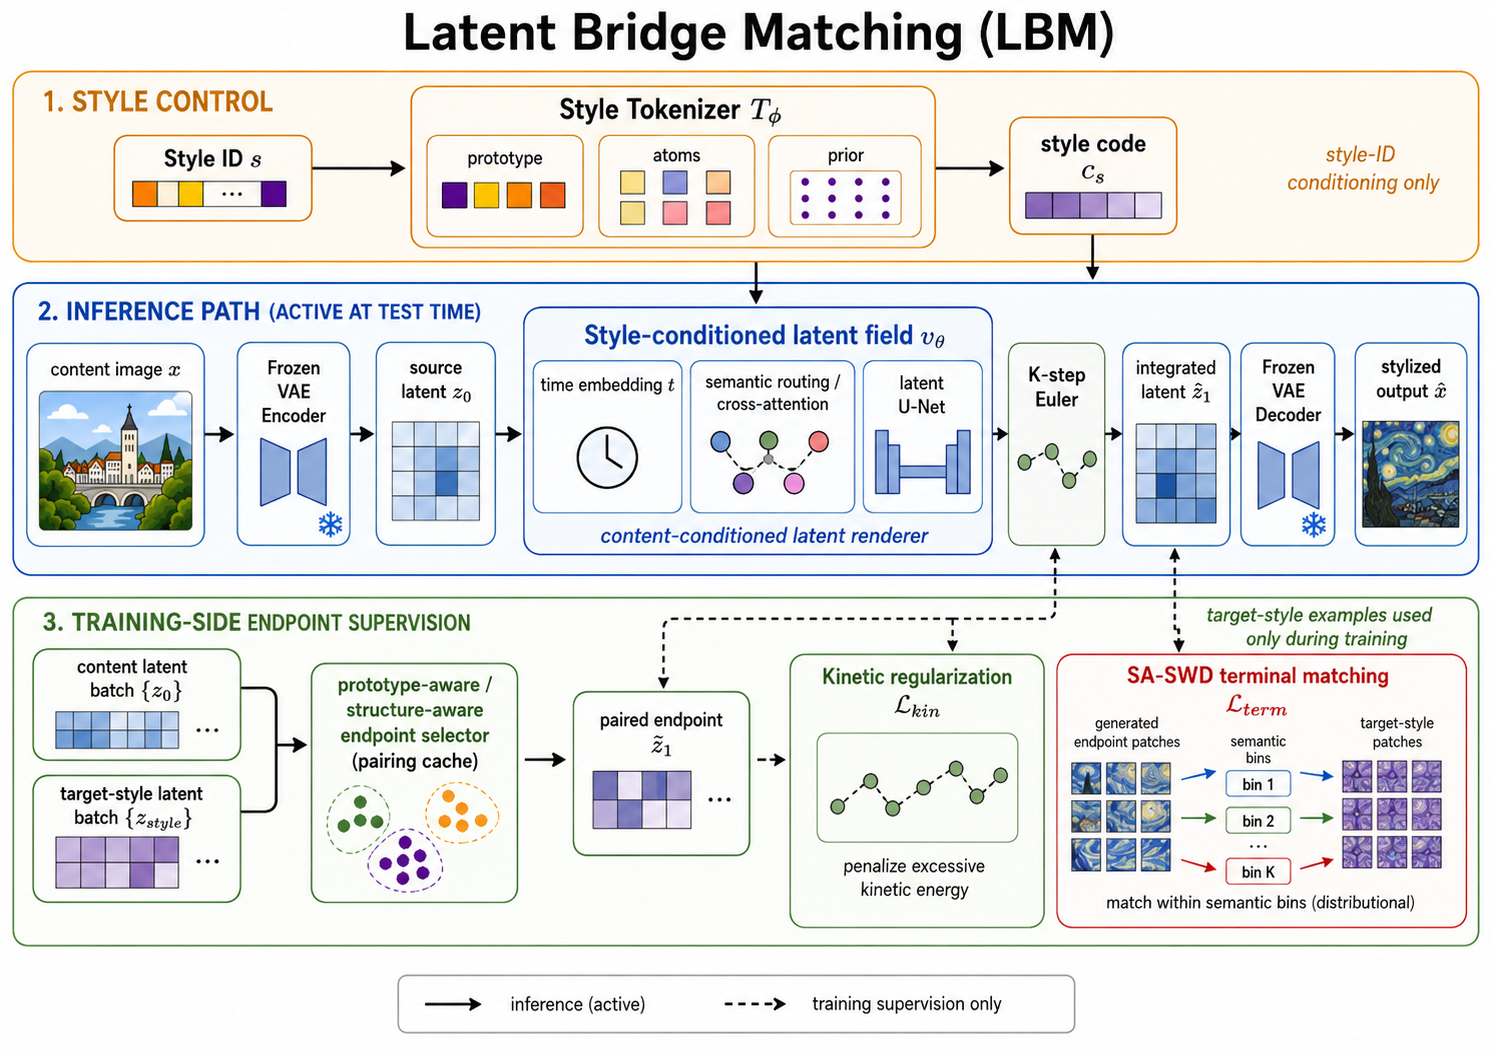
\includegraphics[width=0.54\textwidth]{framework_lbm_main_user.png}
    \caption{LBM in three bands. The top band contains style-ID control only. The middle band is the active test-time latent transport path that must move above the Figure~\ref{fig:distinct5_page1} failure zone and into the frontier. The bottom band contains endpoint construction, kinetic control, and SA-SWD, all used only during training.}
    \label{fig:framework}
\end{figure*}

\section{Experiments}
\subsection{Experimental setup}
We report one main benchmark and one historical secondary packet. Distinct5-WikiArt carries the main claim; the older CycleGAN-256 packet is kept only as secondary support and is never merged into the same leaderboard. Figure~\ref{fig:distinct5_page1} asks whether a compact style-ID family can move above the IDT floor while staying in a usable artifact regime; the rest of this section measures where each row lands on that surface.

\paragraph{Dataset and evaluation metrics.}
Distinct5-WikiArt uses Early Renaissance, Impressionism, Minimalism, Rococo, and Ukiyo-e, with 1000 training images and 30 held-out test images per class. The classes are chosen from WikiArt by a CLIP-style separation screen, and evaluation again uses all $5\times5$ directions over 750 generated images.

The main metrics are transfer CLIP-S, LPIPS, and
\begin{equation}
    \mathrm{EC} = \mathrm{CLIP\mbox{-}style}\cdot(1-\mathrm{LPIPS}).
\end{equation}
For Distinct5-WikiArt we additionally report style gain over the unchanged-image reference,
\begin{equation}
    \Delta_{\mathrm{idt}} = \mathrm{CLIP\mbox{-}S}(\text{method}) - \mathrm{CLIP\mbox{-}S}(\text{idt}),
\end{equation}
under both the full $5\times5$ protocol and the transfer-only off-diagonal subset. On Distinct5, $\Delta_{\mathrm{idt}}$ is the first sanity check: any row at or below zero has failed to move reliably toward the requested target style. EC is used only as a Pareto summary. Auxiliary diagnostics are targetwise ArtFID, a held-out non-CLIP style probe, and standard perceptual/frequency checks \cite{ke2021musiq,yang2022maniqa,ding2020dists,binkowski2018kid}. The historical CycleGAN-256 packet follows the same 750-output protocol and is used only as secondary support later in the paper.

\paragraph{Implementation details.}
All paper-facing LBM rows are trained and evaluated on the reviewed single-lane RTX 3060 WSL surface, and reported train time is cumulative wall-clock to the shown checkpoint with evaluation excluded. Same-cost comparisons therefore align training wall-clock rather than mixed train+eval runtime. Seedream-4.5 is kept only as an external large-prior reference under a fixed API prompt protocol, not as a same-interface style-ID baseline.

\subsection{Main result on Distinct5-WikiArt}
Figure~\ref{fig:distinct5_page1} and Table~\ref{tab:distinct5} give the paper's main result. Distinct5-WikiArt is an IDT-calibrated failure test, not a single-score leaderboard. The unchanged-image control already reaches CLIP-S 0.6801, so any row with $\Delta_{\mathrm{idt}}\le 0$ fails before tradeoff analysis begins.

\paragraph{Quantitative frontier.}
LBM occupies three regimes on that surface: minute-scale anchors, a content-preserving Knee point, and a stronger style band. LBM-K reaches 0.6712 / 0.6277 in transfer CLIP-S / $(1-\mathrm{LPIPS})$, the promoted Knee point reaches 0.7102 / 0.5397, and the stronger successors extend the style side to 0.7274 / 0.3967 and 0.7307 / 0.3817. This is a frontier, not a single winner.

\paragraph{Baseline bounds.}
The reproduced baselines bound that frontier from both sides. SaMST e15 reaches 0.6957 / 0.6319, but in a much higher-damage region, and its retained e5/e15 packet is already near a plateau. Seedream-4.5 is a stronger external large-prior reference, but its transfer row, 0.6920 / 0.4923, still stays below LBM-Knee on both style gain and content preservation. SaMAM-2250 never clears the IDT floor. The latent negatives sharpen the same failure mode: Lat SaMAM stays only +0.0148 above IDT, whereas Lat SaMST collapses to the worst all-pairs ArtFID band at 658.8.

\begin{strip}
\centering
\vspace{-2mm}
\begin{minipage}[t]{0.49\textwidth}
\captionof{table}{Selected Distinct5-WikiArt transfer points. `idt' is the unchanged-image floor. The ordering is deliberate: floor, failed compact baseline, reproduced high-style baselines, compact LBM anchor, closed Knee point, and stronger promoted successors.}
\label{tab:distinct5}
\small
\setlength{\tabcolsep}{3.2pt}
\resizebox{\linewidth}{!}{%
\begin{tabular}{@{}l l r r r l@{}}
\toprule
Point & Role & CLIP-S$_{\mathrm{tr}}\uparrow$ & $1-\mathrm{LPIPS}\uparrow$ & $\Delta_{\mathrm{idt,tr}}\uparrow$ & Closure \\
\midrule
idt & no-op floor & 0.6399 & 1.0000 & 0.0000 & closed \\
SaMAM-2250 & compact baseline & 0.5523 & 0.6395 & -0.0877 & closed \\
SaMST e15 & high-style baseline & 0.6957 & 0.3681 & +0.0558 & closed \\
Seedream-4.5 & large-prior ref. & 0.6920 & 0.5077 & +0.0521 & closed \\
LBM-K e1 & conservative anchor & 0.6712 & 0.6277 & +0.0312 & closed \\
LBM-Knee e13 & content-preserving successor & 0.7102 & \textbf{0.5397} & +0.0703 & closed \\
LBM-PS e13 & balanced high-style & 0.7274 & 0.3967 & +0.0875 & frontier \\
LBM-PS-v2 e13 & style ceiling & \textbf{0.7307} & 0.3817 & \textbf{+0.0908} & frontier \\
\bottomrule
\end{tabular}
}
\end{minipage}\hfill
\begin{minipage}[t]{0.47\textwidth}
\captionof{table}{Artifact-sensitive and non-CLIP diagnostics on selected Distinct5-WikiArt rows. tw-ArtFID uses the all-pairs target-pooled recompute and separates the closed Knee point from the style-ceiling and large-prior rows.}
\label{tab:distinct5_artifact_aux}
\small
\setlength{\tabcolsep}{3.1pt}
\resizebox{\linewidth}{!}{%
\begin{tabular}{@{}l r r r r@{}}
\toprule
Point & tw-ArtFID$_{\mathrm{all}}\downarrow$ & Gram-$\mu\downarrow$ & EdgePurity$\uparrow$ & NonCLIPAcc$\uparrow$ \\
\midrule
LBM-K e1 & 316.5 & 0.153 & \textbf{0.540} & 0.167 \\
LBM-Knee e13 & 388.2 & \textbf{0.137} & 0.288 & 0.237 \\
LBM-PS-v2 e13 & 465.6 & 0.183 & 0.115 & 0.272 \\
SaMST e15 & 395.7 & 0.147 & 0.102 & 0.248 \\
Seedream-4.5 & \textbf{311.5} & 0.189 & 0.389 & \textbf{0.378} \\
\bottomrule
\end{tabular}
}
\end{minipage}
\vspace{-1mm}
\end{strip}

\paragraph{Artifact-sensitive diagnostics.}
Table~\ref{tab:distinct5_artifact_aux} explains why Knee is the promoted default. Against SaMST e15, Knee lowers all-pairs target-pooled ArtFID (388.2 vs.\ 395.7), improves Gram-$\mu$ (0.137 vs.\ 0.147), and more than doubles edge purity (0.288 vs.\ 0.102). The held-out non-CLIP probe keeps Knee close to SaMST (0.237 vs.\ 0.248), while PS-v2 and Seedream move higher on style. Bootstrap keeps both promoted rows safely above IDT, so Knee remains the main closed point and PS-v2 the explicit style ceiling.

\begin{figure*}[t]
    \centering
    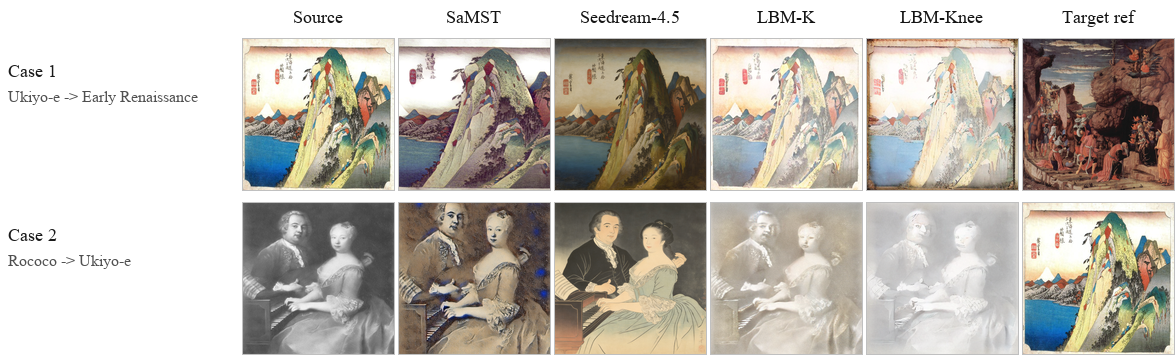
\includegraphics[width=0.985\textwidth]{figures/fig_distinct5_qualitative_main.png}
    \caption{Qualitative reading of Distinct5-WikiArt. Columns are grouped into controls, reproduced baselines, and frontier rows. Panel A shows the calibrated failure mode on `Impressionism $\rightarrow$ Minimalism': plausible outputs can still miss the requested target-style move. Panel B shows the same frontier tradeoff as Figure~\ref{fig:distinct5_page1}: stronger style movement pulls toward SaMST / Seedream / PS-v2, while Knee keeps more of the source layout. Target-domain references are shown only for visualization.}
    \label{fig:qual_main}
\end{figure*}

\paragraph{Qualitative read.}
Figure~\ref{fig:qual_main} shows the same pattern visually. Panel A makes the calibration point concrete: plausible outputs can still miss the requested style move. Panel B shows the grouped frontier itself: high-style baselines and PS-v2 push harder toward the target domain, while LBM-Knee keeps more of the source layout and still moves beyond the compact anchor.

% Evidence-backed timing tables for direct use via:
% % Evidence-backed timing tables for direct use via:
% % Evidence-backed timing tables for direct use via:
% \input{snippets/timing_tables_leibniz}
% ...
% \HistoricalTimingTableLeibniz
% ...
% \DistinctFiveTimingTableLeibniz

\newcommand{\HistoricalTimingTableLeibniz}{%
\begin{table}[t]
\centering
\footnotesize
\setlength{\tabcolsep}{4pt}
\caption{Historical strict-750 / 256$\times$256 recorded operating-point cost. Training time is the wall-clock cost to the manuscript operating point; inference is the end-to-end runtime for the 750-image protocol. This is recorded operating-point context, not a normalized time-to-quality comparison.}
\label{tab:cost}
\begin{tabular}{@{}lccc@{}}
\toprule
Method & Train to point & Infer-750 & ms/img \\
\midrule
LBM & \textbf{5.2 min} & 85.4 s & 114 \\
\bottomrule
\end{tabular}

\vspace{2pt}
\parbox{0.98\linewidth}{\raggedright\footnotesize\textit{Note.} The LBM row is a preserved timing record. Other historical rows are intentionally omitted here because the available train/infer evidence is either probe-estimated, mixed-protocol, or incomplete rather than a closed operating-point packet.}
\end{table}%
}

\newcommand{\DistinctFiveTimingTableLeibniz}{%
\begin{table}[t]
\centering
\footnotesize
\setlength{\tabcolsep}{4pt}
\caption{Distinct5-512 recorded operating-point cost under the reviewed full $5\times5$ / 750-output packet. Reported train time is cumulative training wall-clock to the shown checkpoint, with evaluation excluded. This is recorded operating-point cost, not a normalized time-to-quality comparison.}
\label{tab:cost_distinct5}
\begin{tabular}{@{}lcc@{}}
\toprule
Method & Recorded point & Train to point \\
\midrule
LBM-F & e1 & \textbf{1.2 min} \\
LBM-K & e1 & \textbf{1.2 min} \\
SaMAM & step 2250 & 7.6 h \\
SaMST & e15 & 5.8 h \\
\bottomrule
\end{tabular}

\vspace{2pt}
\parbox{0.98\linewidth}{\raggedright\footnotesize\textit{Note.} Distinct5 times are cumulative training wall only, with evaluation excluded. We intentionally omit a shared inference column because same-grade pure-generation timing is still incomplete for the active manuscript rows \texttt{SaMAM-2250} and \texttt{SaMST-e15}; leaving blanks would overstate closure. Post-2250 SaMAM timings are intentionally excluded.}
\end{table}%
}

% ...
% \HistoricalTimingTableLeibniz
% ...
% \DistinctFiveTimingTableLeibniz

\newcommand{\HistoricalTimingTableLeibniz}{%
\begin{table}[t]
\centering
\footnotesize
\setlength{\tabcolsep}{4pt}
\caption{Historical strict-750 / 256$\times$256 recorded operating-point cost. Training time is the wall-clock cost to the manuscript operating point; inference is the end-to-end runtime for the 750-image protocol. This is recorded operating-point context, not a normalized time-to-quality comparison.}
\label{tab:cost}
\begin{tabular}{@{}lccc@{}}
\toprule
Method & Train to point & Infer-750 & ms/img \\
\midrule
LBM & \textbf{5.2 min} & 85.4 s & 114 \\
\bottomrule
\end{tabular}

\vspace{2pt}
\parbox{0.98\linewidth}{\raggedright\footnotesize\textit{Note.} The LBM row is a preserved timing record. Other historical rows are intentionally omitted here because the available train/infer evidence is either probe-estimated, mixed-protocol, or incomplete rather than a closed operating-point packet.}
\end{table}%
}

\newcommand{\DistinctFiveTimingTableLeibniz}{%
\begin{table}[t]
\centering
\footnotesize
\setlength{\tabcolsep}{4pt}
\caption{Distinct5-512 recorded operating-point cost under the reviewed full $5\times5$ / 750-output packet. Reported train time is cumulative training wall-clock to the shown checkpoint, with evaluation excluded. This is recorded operating-point cost, not a normalized time-to-quality comparison.}
\label{tab:cost_distinct5}
\begin{tabular}{@{}lcc@{}}
\toprule
Method & Recorded point & Train to point \\
\midrule
LBM-F & e1 & \textbf{1.2 min} \\
LBM-K & e1 & \textbf{1.2 min} \\
SaMAM & step 2250 & 7.6 h \\
SaMST & e15 & 5.8 h \\
\bottomrule
\end{tabular}

\vspace{2pt}
\parbox{0.98\linewidth}{\raggedright\footnotesize\textit{Note.} Distinct5 times are cumulative training wall only, with evaluation excluded. We intentionally omit a shared inference column because same-grade pure-generation timing is still incomplete for the active manuscript rows \texttt{SaMAM-2250} and \texttt{SaMST-e15}; leaving blanks would overstate closure. Post-2250 SaMAM timings are intentionally excluded.}
\end{table}%
}

% ...
% \HistoricalTimingTableLeibniz
% ...
% \DistinctFiveTimingTableLeibniz

\newcommand{\HistoricalTimingTableLeibniz}{%
\begin{table}[t]
\centering
\footnotesize
\setlength{\tabcolsep}{4pt}
\caption{Historical strict-750 / 256$\times$256 recorded operating-point cost. Training time is the wall-clock cost to the manuscript operating point; inference is the end-to-end runtime for the 750-image protocol. This is recorded operating-point context, not a normalized time-to-quality comparison.}
\label{tab:cost}
\begin{tabular}{@{}lccc@{}}
\toprule
Method & Train to point & Infer-750 & ms/img \\
\midrule
LBM & \textbf{5.2 min} & 85.4 s & 114 \\
\bottomrule
\end{tabular}

\vspace{2pt}
\parbox{0.98\linewidth}{\raggedright\footnotesize\textit{Note.} The LBM row is a preserved timing record. Other historical rows are intentionally omitted here because the available train/infer evidence is either probe-estimated, mixed-protocol, or incomplete rather than a closed operating-point packet.}
\end{table}%
}

\newcommand{\DistinctFiveTimingTableLeibniz}{%
\begin{table}[t]
\centering
\footnotesize
\setlength{\tabcolsep}{4pt}
\caption{Distinct5-512 recorded operating-point cost under the reviewed full $5\times5$ / 750-output packet. Reported train time is cumulative training wall-clock to the shown checkpoint, with evaluation excluded. This is recorded operating-point cost, not a normalized time-to-quality comparison.}
\label{tab:cost_distinct5}
\begin{tabular}{@{}lcc@{}}
\toprule
Method & Recorded point & Train to point \\
\midrule
LBM-F & e1 & \textbf{1.2 min} \\
LBM-K & e1 & \textbf{1.2 min} \\
SaMAM & step 2250 & 7.6 h \\
SaMST & e15 & 5.8 h \\
\bottomrule
\end{tabular}

\vspace{2pt}
\parbox{0.98\linewidth}{\raggedright\footnotesize\textit{Note.} Distinct5 times are cumulative training wall only, with evaluation excluded. We intentionally omit a shared inference column because same-grade pure-generation timing is still incomplete for the active manuscript rows \texttt{SaMAM-2250} and \texttt{SaMST-e15}; leaving blanks would overstate closure. Post-2250 SaMAM timings are intentionally excluded.}
\end{table}%
}

\DistinctFiveTimingTableLeibniz

\paragraph{Retest and cost.}
The same ordering survives direct reevaluation and cost comparison. Under explicit three-scope retest, Knee reaches 0.7101 / 0.4604 on transfer and 0.7302 / 0.4560 on all-pairs in CLIP-S / LPIPS, versus 0.6920 / 0.4923 and 0.7198 / 0.4767 for Seedream-4.5. Table~\ref{tab:cost_distinct5} then shows why that row matters in practice: conservative LBM anchors cross the Distinct5-WikiArt IDT floor after 1.2 minutes on a single RTX 3060, whereas SaMAM-2250 remains below the floor after 7.6 hours and SaMST exceeds it only after 5.8 hours in a much higher-damage region. The family is therefore selectable rather than singular: LBM-K is the conservative anchor, LBM-Knee the default closed point, and PS-v2 the style-ceiling row.

\subsection{Historical support and secondary evidence}
We keep the historical CycleGAN-256 packet only as secondary support. On that older surface, LBM remains a competitive compact retrainable point at 0.7161 CLIP-S / 0.4514 LPIPS and 114\,ms/image, while the strongest reproduced competitors either collapse content or enter noisier artifact regimes. Two fixed-rule WikiArt follow-up splits preserve the same evaluator pattern: unchanged images still score strongly, and compact LBM-F remains above the split-local IDT floor by `+0.0139` and `+0.0073` transfer CLIP-S. The supplement carries the artifact ledger and protocol details.



\section{Discussion and Limitations}
The main lesson is not that one row wins every metric; it is that Distinct5-WikiArt is easy to misread. Raw CLIP-style overstates success in art-to-art transfer. Once the unchanged-image floor is explicit, several reproduced baselines stop counting as evidence of target-style control: some never beat the unchanged image, while others do so only by entering substantially worse LPIPS and artifact regions. The benchmark then exposes a compact frontier: low-damage anchors, a closed Knee point, and a stronger style-ceiling regime.

The limitations are direct. The task is domain-level rather than exemplar-level, Euler integration is intentionally simple, and artifact-sensitive diagnostics are still proxies rather than preference judgments. Distinct5-WikiArt is a stress benchmark rather than a universal art benchmark, although the fixed-rule follow-up splits reproduce the same unchanged-image pathology.

\section{Conclusion}
IDT calibration changes what counts as success in domain-level art transfer. Once the unchanged-image prior is measured explicitly, compact latent transport is enough to produce useful style-ID operating points: minute-scale anchors, a closed Knee point, and a stronger style-ceiling regime. LBM therefore offers a practical small-model alternative to large-prior adaptation on Distinct5-WikiArt.

\bibliography{refs}

\footnotesize
\setlength{\itemsep}{0pt}
\setlength{\parskip}{1pt}
\section*{Reproducibility Checklist}
\noindent\textbf{This paper}
\begin{itemize}
\item Includes a conceptual outline and/or pseudocode description of AI methods introduced: \textbf{Yes}.
\item Clearly delineates statements that are opinions, hypothesis, and speculation from objective facts and results: \textbf{Yes}.
\item Provides well marked pedagogical references for less-familiar readers to gain background necessary to replicate the paper: \textbf{Yes}.
\end{itemize}

\noindent\textbf{Does this paper make theoretical contributions?} \textbf{Yes (design-grounding)}. The paper provides compact formal analysis with proofs and empirical checks: Theorem~1 and Theorem~2 analyze the active field/solver regime through a path-action decomposition for kinetic regularization and an $O(1/K)$ Euler discretization bound, while Theorem~3 analyzes a historical OT-style assignment variant as family-level background. Full proofs are in the supplement. These results justify the three-part design without asserting equivalence to a full Schr\"odinger Bridge solver.

\noindent\textbf{Does this paper rely on one or more datasets?} \textbf{Yes}.
\begin{itemize}
\item A motivation is given for why the experiments are conducted on the selected datasets: \textbf{Yes}.
\item All novel datasets introduced in this paper are included in a data appendix: \textbf{NA}.
\item All novel datasets introduced in this paper will be made publicly available upon publication of the paper with a license that allows free usage for research purposes: \textbf{NA}.
\item All datasets drawn from the existing literature are accompanied by appropriate citations: \textbf{Yes}.
\item All datasets drawn from the existing literature are publicly available: \textbf{Yes}.
\item All datasets that are not publicly available are described in detail, with explanation why publicly available alternatives are not scientifically satisficing: \textbf{NA}.
\end{itemize}

\noindent\textbf{Does this paper include computational experiments?} \textbf{Yes}.
\begin{itemize}
\item This paper states the number and range of values tried per (hyper-)parameter during development of the paper, along with the criterion used for selecting the final parameter setting: \textbf{Partial}.
\item Any code required for pre-processing data is included in the appendix: \textbf{Partial} (the supplement lists the reviewed script paths and artifact roots for the current paper-facing packets).
\item All source code required for conducting and analyzing the experiments is included in a code appendix: \textbf{Partial} (the supplement enumerates the main reviewed scripts, configs, and eval artifacts, but does not inline the full codebase).
\item All source code required for conducting and analyzing the experiments will be made publicly available upon publication of the paper with a license that allows free usage for research purposes: \textbf{Partial}.
\item All source code implementing new methods have comments detailing the implementation, with references to the paper where each step comes from: \textbf{Partial}.
\item If an algorithm depends on randomness, then the method used for setting seeds is described in a way sufficient to allow replication of results: \textbf{Partial} (the supplement records the reviewed seed settings for the current paper-facing packets, but external references such as Seedream do not expose a user-controlled seed).
\item This paper specifies the computing infrastructure used for running experiments, including hardware/software details: \textbf{Yes}.
\item This paper formally describes evaluation metrics used and explains the motivation for choosing these metrics: \textbf{Yes}.
\item This paper states the number of algorithm runs used to compute each reported result: \textbf{Yes}.
\item Analysis of experiments goes beyond single-dimensional summaries of performance to include measures of variation, confidence, or other distributional information: \textbf{Yes}.
\item The significance of any improvement or decrease in performance is judged using appropriate statistical tests: \textbf{Partial} (selected confidence intervals and bootstrap summaries are reported, but not every manuscript comparison is presented as a closed significance claim).
\item This paper lists all final (hyper-)parameters used for each model/algorithm in the paper's experiments: \textbf{Partial}.
\end{itemize}

\end{document}



